\chapter{A Software Framework for Machine Learning-Based Solutions for HPC Optimization}
\label{OverviewSolution.ch}

In this section, we present two approaches for delivering AI-driven solutions as a stack of applications and software aimed at addressing the key research questions and current challenges outlined in Chapters \ref{Sec:Problem_KeyReserachQuestions} and \ref{Background.ch}.

\begin{itemize}
    \item \textbf{Solution1:} We propose the \textbf{HPC Application Resource Estimator (HARP)} — a framework designed to generate job-specific profiling data for training off-the-shelf and custom resource (runtime) prediction models using custom loss functions. HARP dynamically selects the optimal model per application at a given instance for inference. 
    \item \textbf{Solution2:} We propose the \textbf{Smart Scheduler Framework}, which leverages a the estimation models developed in HARP and a \textbf{CI database} to create and execute jobs using a \textbf{job monitoring daemon}.
\end{itemize}


\begin{figure}[h]
    \centering
    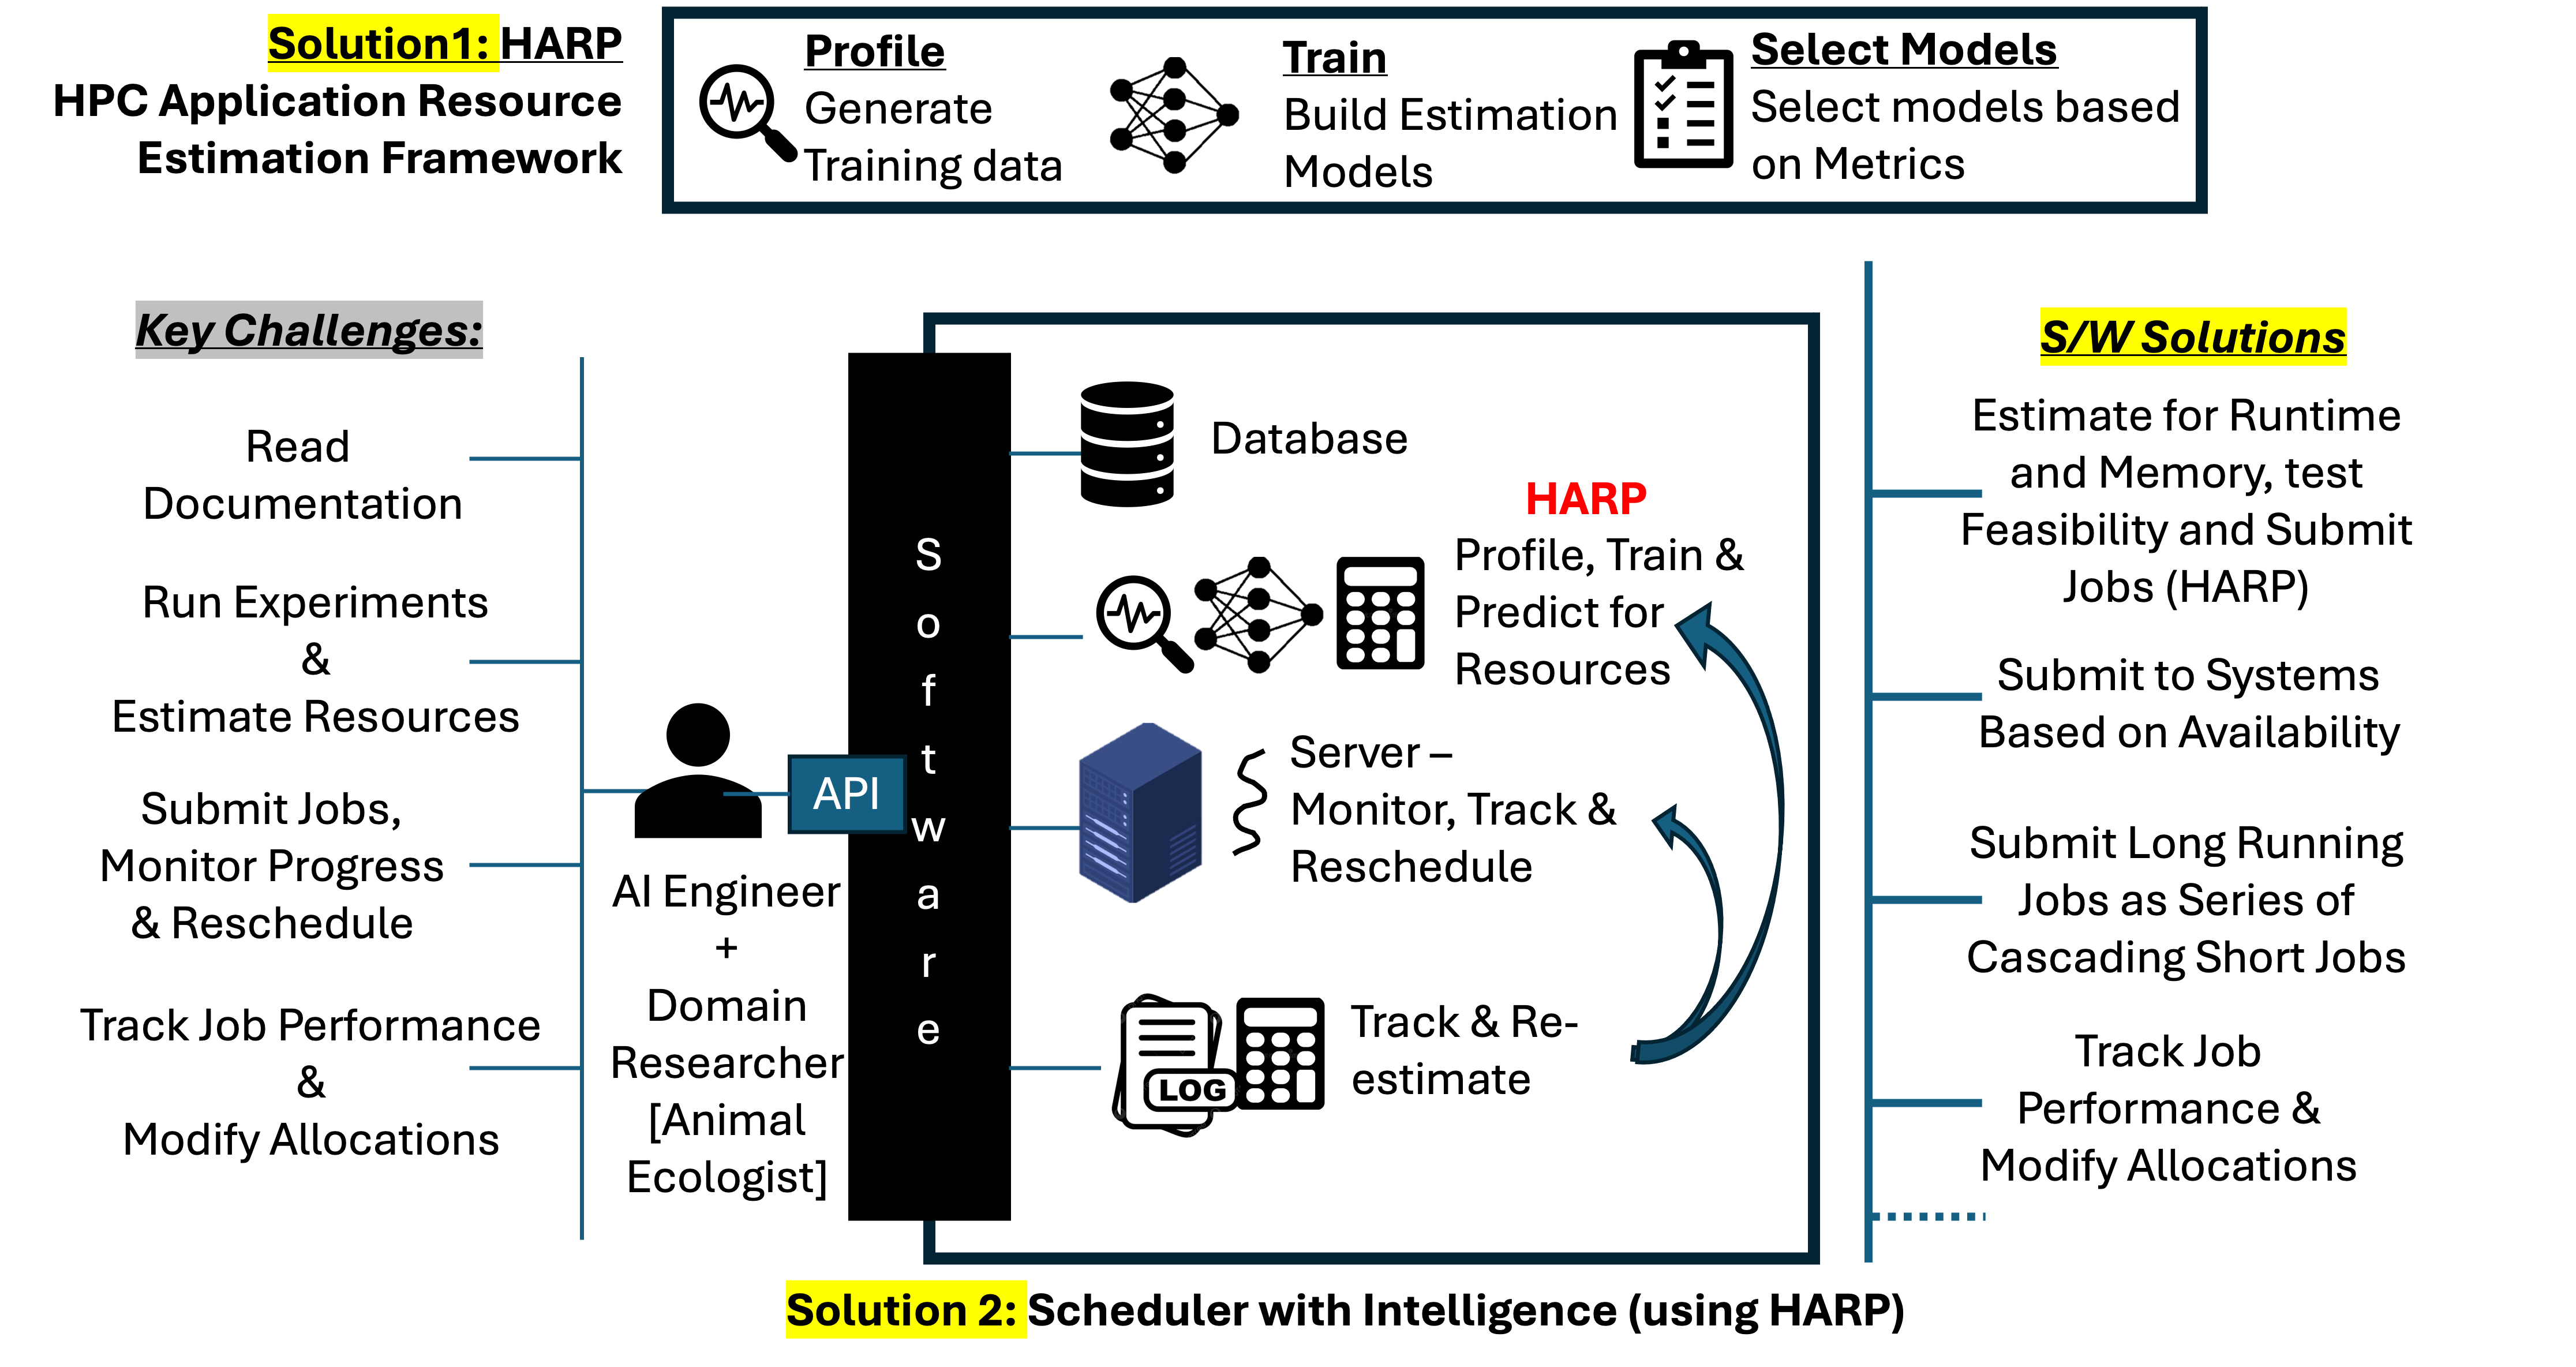
\includegraphics[width=1.0\textwidth]{Images/Solution.png}
    \caption{Software-Driven Solutions for HPC Resource Optimization.}
    \label{fig:hpc_solutions}
\end{figure}

Figure \ref{fig:hpc_solutions} illustrates the key components developed to address the research questions outlined in Chapter \ref{problem.ch}. It highlights Solution 1 (HARP)—an AI-driven framework for workload profiling, training data curation, and building and selecting application-specific runtime estimators. Additionally, it presents Solution 2 (Smart Scheduler), which focuses on job scheduling, monitoring, and automation to enhance HPC resource management.

\paragraph{Modular Software Component Perspective}
The above solutions are designed as a stack of modular components, enabling reuse across various end-to-end implementations.

\begin{enumerate}
    \item \textbf{Cyberinfrastructure Database} – A structured database, derived from \textbf{CI documentation and hardware configurations}, is utilized in HARP to retrieve system configurations and in the Scheduler to plan execution. See Section \ref{Sec:CIDatabase} for further details.
    \item \textbf{Generating Training Data} – \textbf{Offline profiling of workloads} to create datasets for training resource estimators.  Refer to Chapter \ref{GenerateData.ch} for details on training data generation and its characteristics. The data generation pipeline can be utilized for producing training data for HARP, obtaining inference data in the Scheduler, or in future work where the Intelligence Plane emulates workflows in new environments to adapt predictions to different systems or configurations.
    \item \textbf{Building Regression Models} – A \textbf{pipeline for training resource estimation models}, which can either \textbf{auto-schedule jobs} or \textbf{validate user-provided resource requests}. Refer to Chapter \ref{BuildEstimator.ch} for an understanding of the loss functions and metrics used in training resource (walltime) estimators, as well as the process of selecting an estimation model to infer runtimes for a targeted application.
    \item \textbf{Intelligent Scheduler (Intelligence Plane)} – A framework that \textbf{automates job submission, monitoring, tracking, and rescheduling}, ensuring jobs run \textbf{to completion} efficiently. Refer to Section \ref{iSchedulerF} for an overview of the architecture, and to Sections \ref{usecase_trainresnet} and \ref{uesecase_trainmegadetector} in Chapter \ref{UseCase.ch} for insights into the framework's operation.  
 
\end{enumerate}

\noindent
These solutions aim to \textbf{reduce inefficiencies, improve resource utilization, and automate job management} in HPC environments.  



\section{HARP - The HPC Application Resource Estimation Framework}
\label{HARP}
In this section, we describe the three components - "generate", "build" and "predict" - that form the heart of HARP. 

\begin{figure}[h]
  \centering
  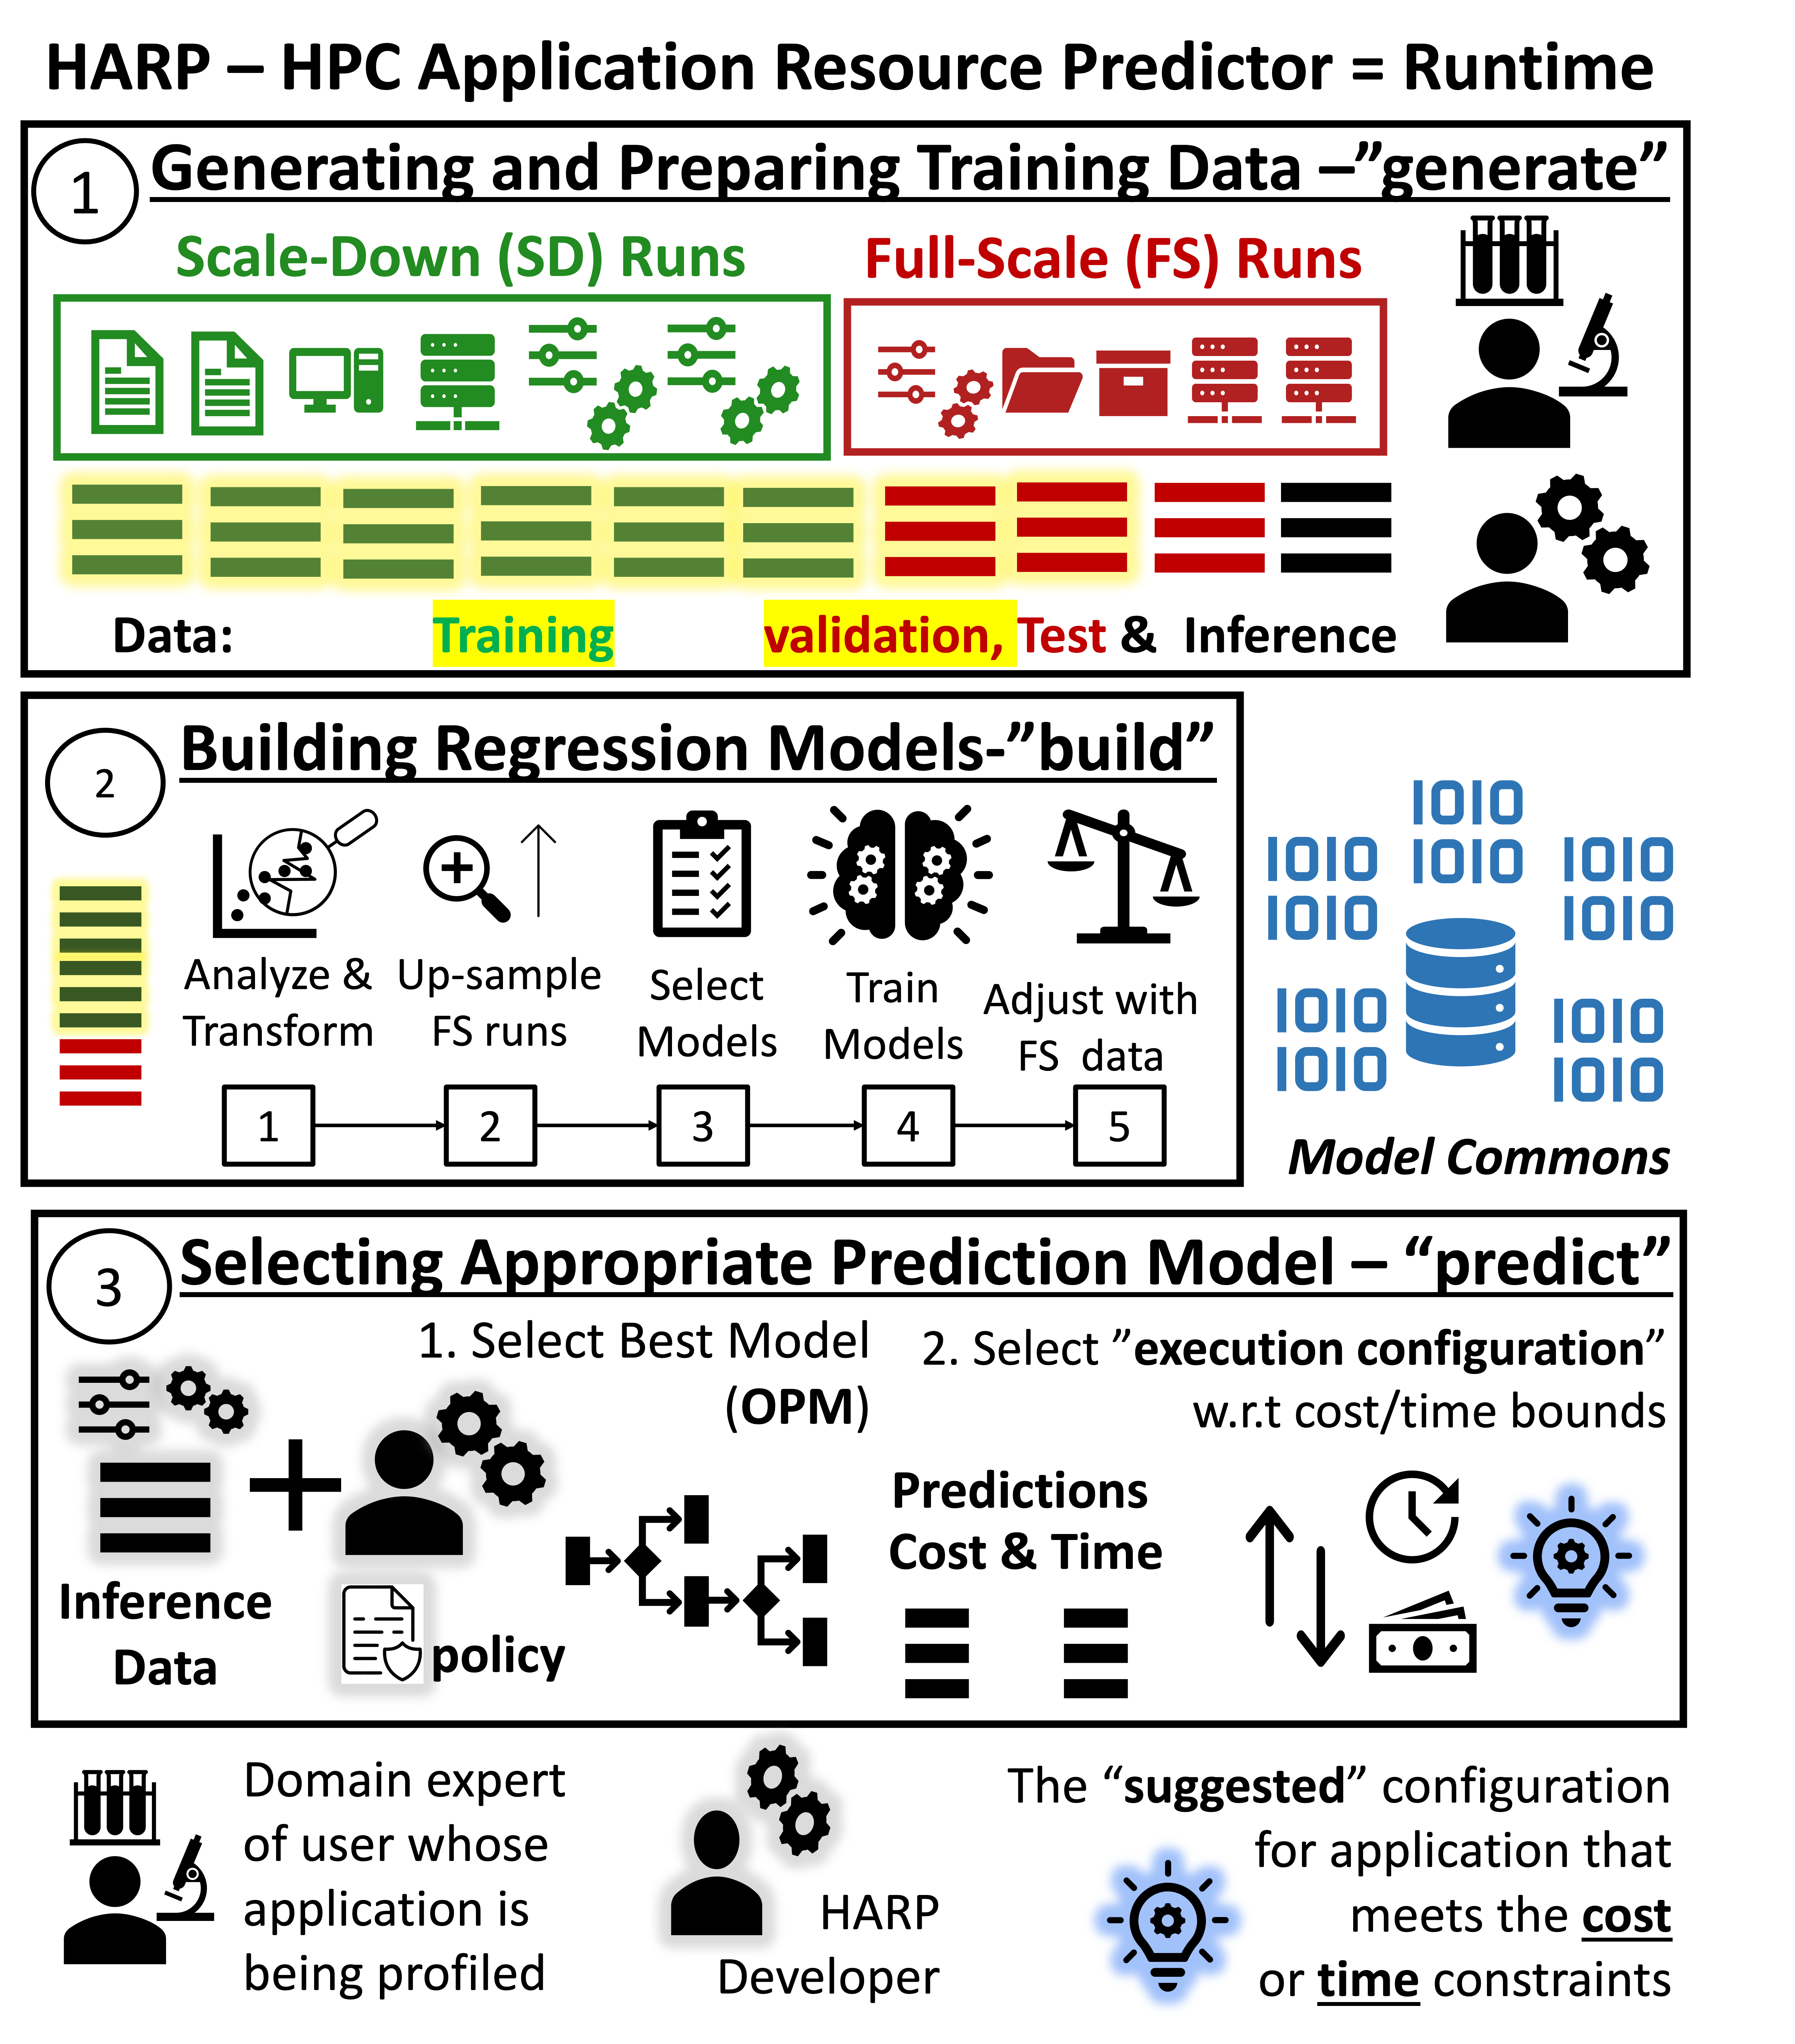
\includegraphics[width=12cm, height=10cm]{Images/HARP_Pipeline.png}
  \caption{Visualizing the Automated Data Collection Pipeline and Model Generation}
  \Description{the Automated Data Collection Pipeline built using Cheetah, TAU, and model generation}
  \label{fig:HARP_pipeline}
\end{figure}

\begin{enumerate}
  \item \textbf{The Human-in-the-Loop "Generate" Component:}  
  Utilizing the CODAR Framework \footnote{https://github.com/CODARcode/cheetah}, this component generates training data by executing applications under scaled-down (SD) and full-scale (FS) configurations. The HARP user defines application-specific hyperparameters and profiling endpoints to generate training data tailored to these configurations.  

  The SD configurations are designed to capture a diverse range of tunable workload characteristics, such as different input types and batch sizes for neural networks, and serve as primary training data. In contrast, FS configurations represent actual workload characteristics, such as the expected batch size recommended by the research community, and are primarily used to validate or test "seen/unseen feature" estimations.  

  As FS workloads become available from user history, they can be incrementally added to the training data, improving model adaptability to real-world workloads. SD executions run applications at a smaller scale, producing lighter and faster workloads, allowing efficient testing across a broad range of applications and allocation configurations. FS runs, on the other hand, scale this information to larger input sizes and hardware configurations, ensuring the model generalizes effectively.  

  Chapter \ref{GenerateData.ch} provides an in-depth understanding of application-specific training data generation with user feedback in the loop, along with several application-centric examples illustrating its implementation.

  \item \textbf{The Automated "Build" Component:}  
  This component processes the generated training data by capturing all relevant features that influence walltime estimation. These features can include unknown contributors (e.g., memory affecting core allocation per node, which in turn impacts execution time) and presumed features (e.g., `omp-num-threads` and cores allocated per node), which may introduce redundancy.  

  The build component pre-processes training data by removing redundant features and combining correlated features to reduce dimensionality and enhance predictive model accuracy. Different regression models—Multi-Layer Perceptron (MLP), Decision Tree Regressor (DTR), and Simple Neural Network Regressor (NNR)—are trained using pre-processed data with various combinations of training datasets (SD, SD+n\%FS) and stored for inference.  

  The models are continually trained with incremental FS sample generation (\%FS), simulating human learning. To address SD-FS imbalances, FS data is upsampled, and predictions are scaled against the FS validation dataset using an adjustment factor.

  \item \textbf{The Policy-Driven "Predict" Component:}  
  The final component of the framework predicts execution time for inference (test data). The best-performing model is selected using the Mean Absolute Error (MAE) metric or a custom policy that balances under-prediction and over-estimation, incorporating multiple evaluation metrics such as under-prediction percentage (UPP) and over-estimation mean absolute percentage error (OE\_MAPE).  

  A model performs optimally when it minimizes UPP while reducing OE\_MAPE. Based on this policy, the framework selects the Optimal Predictive Model (OPM) and estimates walltime across all available configurations (hardware and application). The final allocation configuration is then determined based on time and cost constraints, ensuring optimal resource usage.

\end{enumerate}

Chapter \ref{GenerateData.ch} outlines all data pre-processing techniques, while Chapter \ref{BuildEstimator.ch} details model training for runtime estimations, enabling the dynamic selection of the optimal estimation model based on the characteristics of the application (i.e., the generated training data).



\section{iScheduler - The Smart Scheduler Framework }
\label{iSchedulerF}
With a diverse range of estimation models and techniques available, as outlined in Chapter \ref{Background.ch}, it is essential to develop a framework that enables users to interact with these models effectively. However, accessing and utilizing these models remains a challenge for end-users who request resources and schedule jobs, primarily due to the lack of reproducible code or ready-to-use components. To our knowledge, no existing framework seamlessly integrates these models to automate end-to-end job orchestration from development to execution. To address this gap, we propose a smart-scheduler framework, \textbf{iScheduler}, designed to orchestrate job execution by leveraging AI-driven resource allocation models. This framework facilitates job monitoring and scheduling through helper functions and API calls, enabling seamless interaction with HPC centers and improving the efficiency of resource provisioning.

\begin{figure}[ht]
    \centering
    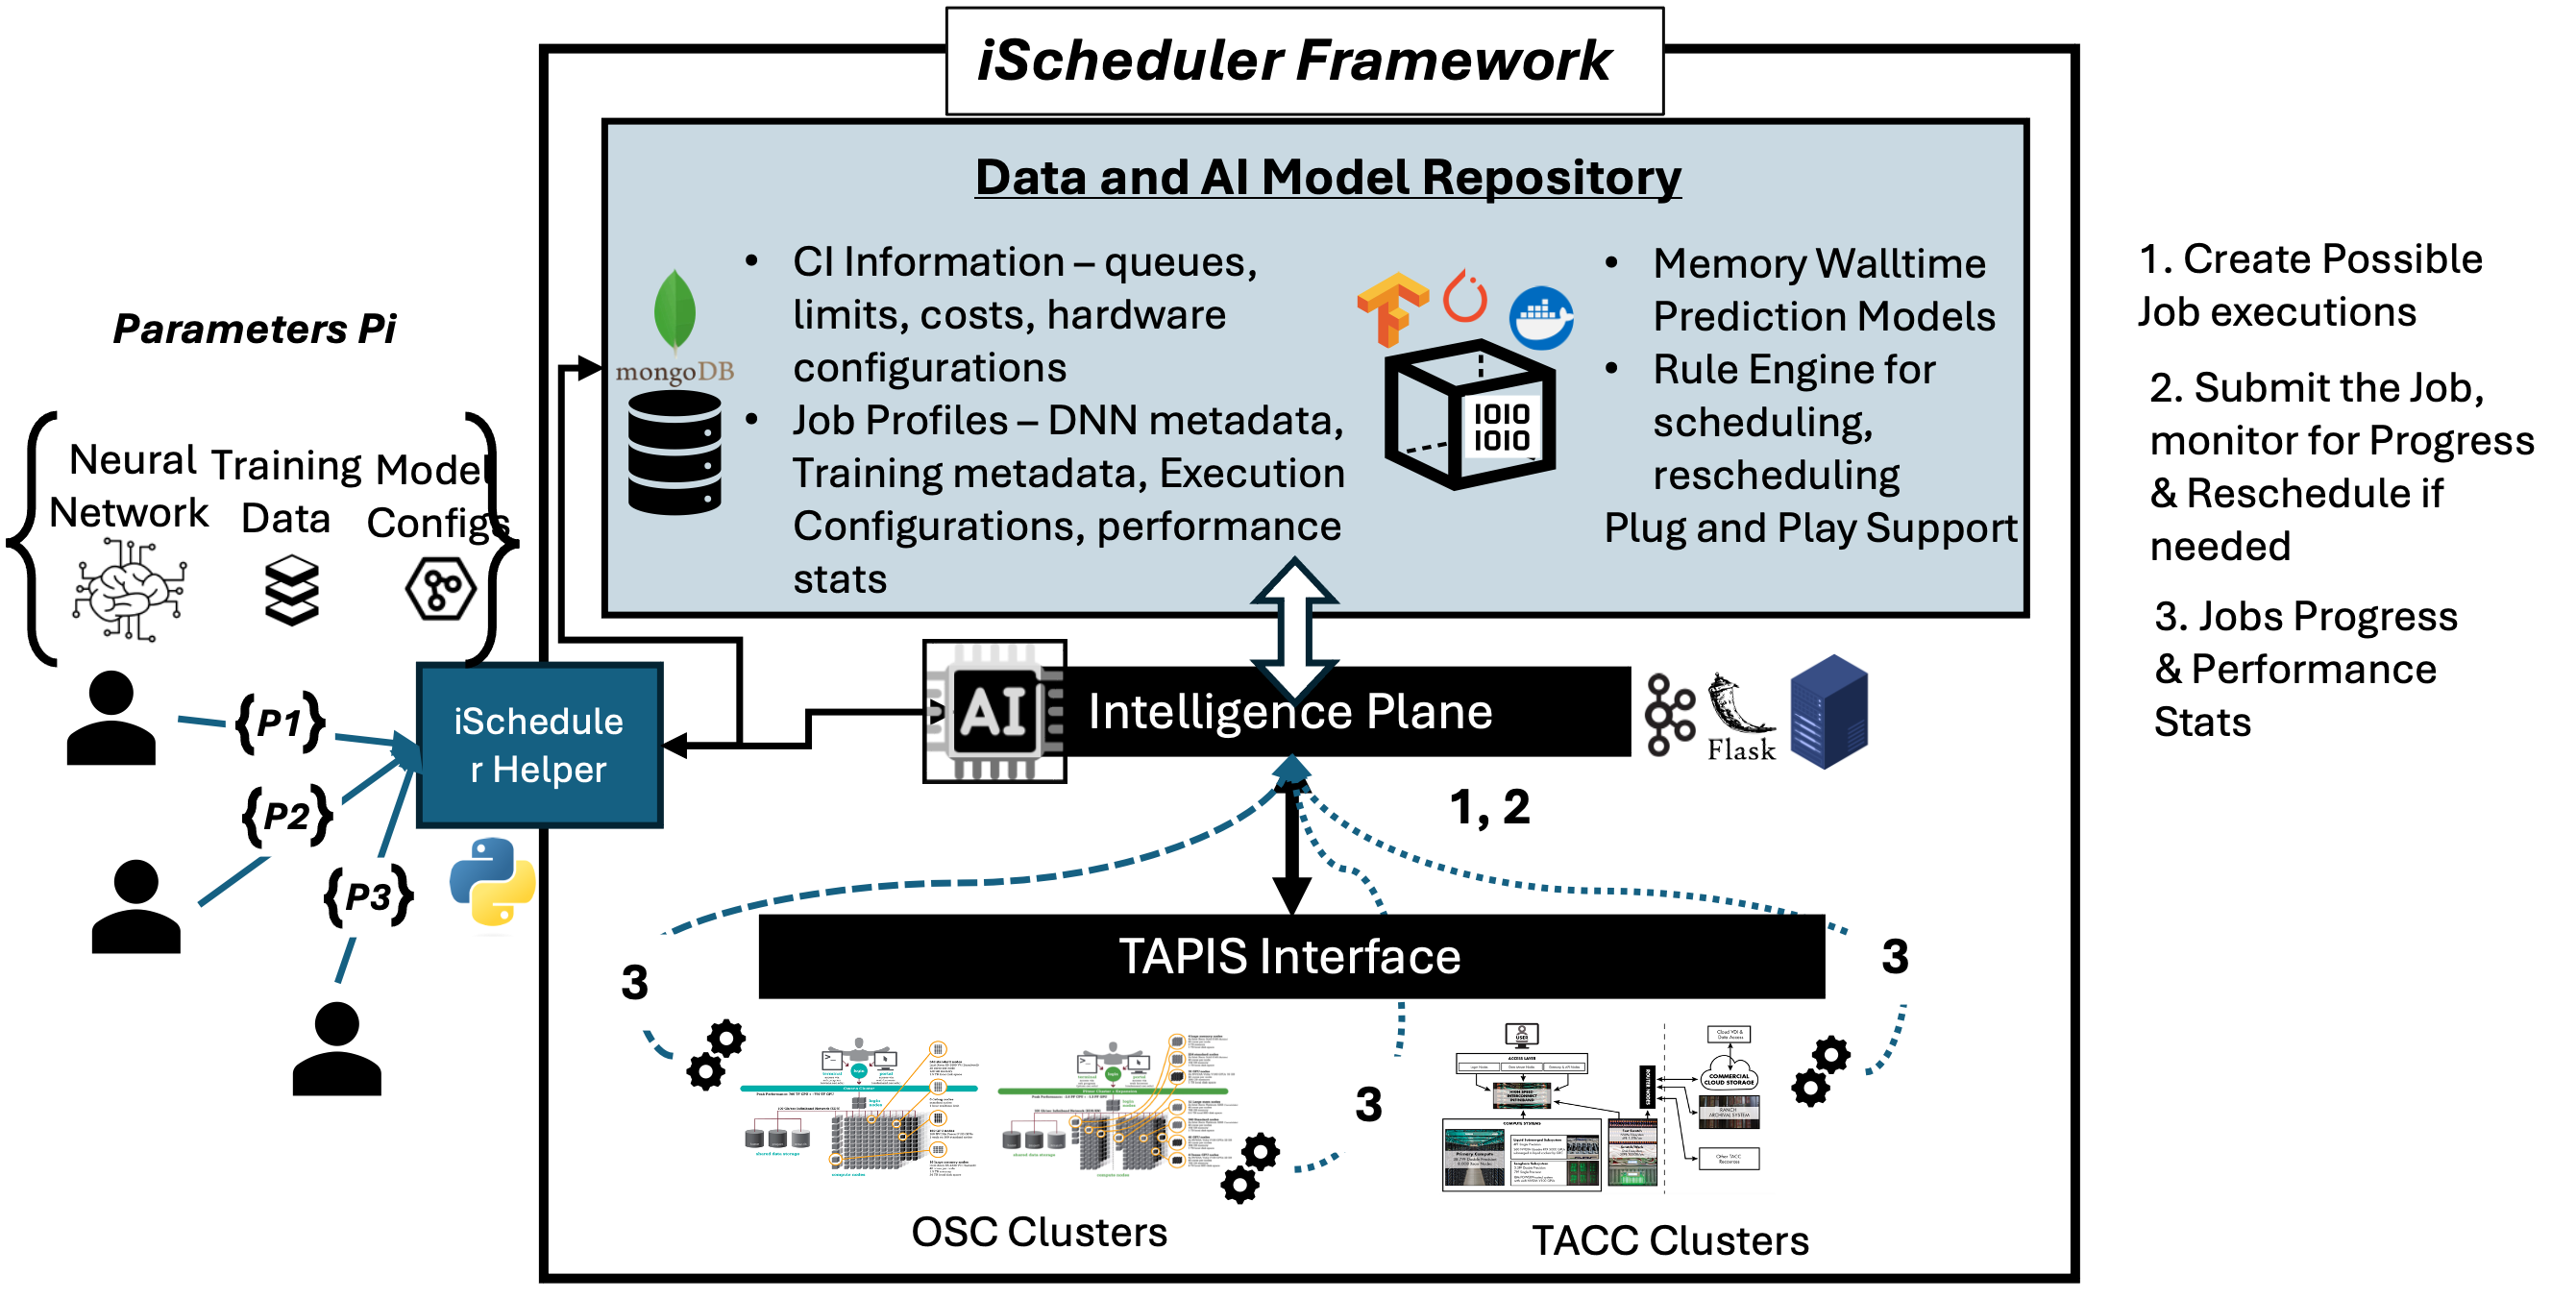
\includegraphics[width=\textwidth]{Images/IScheduler.png}
    \caption{Overview of the iScheduler Framework. The framework integrates an AI-powered Intelligence Plane for resource provisioning and scheduling. It leverages a data and AI model repository containing job profiles, execution configurations, and walltime prediction models. The iScheduler Helper, implemented in Python, interacts with TAPIS  for execution management.}
    \label{fig:iScheduler}
\end{figure}

The iScheduler Framework (as shown in Figure \ref{fig:iScheduler}) has the following components to orchestrate their jobs:
\begin{itemize}
    \item Provides an end-user helper tool, a iScheduler Helper Python module, to interact with cloud-hosted estimators for fetching resource requirements and orchestrating job submissions. 
    \item Utilizes a CI database (DB) to store system information and policies, aiding predictions and decision-making before job submission.\footnote{We used the CI documentation and SLURM commands to create the DB}. 
    \item Returns list of feasible predictions (walltime), execution status, and cost feasibility against available systems to end users, enabling them to either submit jobs manually or delegate them (via Intelligence Plane).
    \item Includes an Intelligence Plane (IP) Service for job submission, monitoring, and tracking on behalf of the user (using TAPIS APIs \cite{stubbs2021tapis})
    \item Supports plug-and-play upgrades to AI estimators (deployed as container images and executed as TAPIS apps or deployed on ML inference server ).
\end{itemize}


\section{Cyberinfrastructure (CI) Database: Structure, Implementation, and Applications}
\label{Sec:CIDatabase}

This section introduces the Cyberinfrastructure (CI) Database, detailing its development, architecture, and role in HPC batch submission optimization. The CI Database serves as a centralized repository that stores all necessary information to assist users in creating feasible batch scripts, optimizing resource allocation, and estimating execution costs. As the foundation of intelligent job scheduling, it enables data-driven allocation decisions, execution planning, and feasibility validation.

To enhance accessibility, the CI Database Interface integrates billing formulas and resource allocation policies, ensuring accurate cost estimations. It applies costing models based on supercomputing center policies:
\begin{itemize}
    \item OSC (Ohio Supercomputer Center): Uses Resource Units (RUs), billing based on CPU and GPU allocations, allowing node sharing.
    \item TACC (Texas Advanced Computing Center): Uses Service Units (SUs), billing per entire node allocation, as node sharing is not permitted.
\end{itemize}

\subsection{Sources of Information for Building the CI Database}
The CI database is primarily constructed by scraping supercomputing center cluster webpages, such as OSC - Pitzer \footnote{https://www.osc.edu/resources/technical\_support/supercomputers/pitzer} and TACC - Frontera \footnote{https://docs.tacc.utexas.edu/hpc/frontera/}. However, the information available on these pages is often limited—for instance, they may not list all available system queues. To address this, we utilize a system development tool \footnote{https://github.com/ICICLE-ai/sysdef\_tool} to extract detailed system information, including all available queues, CI limitations, and other relevant factors. This tool is executed from cluster login nodes to retrieve node configurations, while additional details, such as client billing costs, are fetched directly from the respective supercomputing center websites.

\subsubsection{Supercomputing Center Websites}
These sources provide costing policies per queue, including details on resource units (RUs/SUs), billing policies, and hardware configurations. Example costing from TACC: A Lonestar6 A100 node equipped with three GPUs incurs a cost of 4 Service Units (SUs) per node-hour, while a Lonestar6 H100 node with two GPUs costs 6 SUs per node-hour. The minimum billing period for both configurations is 15 minutes (0.25 hours). For a 48-hour full allocation, an A100 node would require 192 SUs (\(4 \times 48\)), whereas an H100 node would cost 288 SUs (\(6 \times 48\)). If a job is terminated early, before completing the minimum 15-minute billing period, the cost would be 1 SU for an A100 node (\(4 \times 0.25\)) and 1.5 SUs for an H100 node (\(6 \times 0.25\)). These calculations help estimate resource costs and optimize job scheduling based on computational requirements and system constraints. The CI Database integrates this information to estimate costs dynamically based on predicted walltime and system feasibility.

\subsubsection{SLURM Interface}
As discussed in Chapter \ref{Background.ch}, Section \ref{sec:SLURM}, SLURM provides a range of databases that users can query to retrieve relevant information, such as the number of jobs in a queue, the status of their submitted jobs, and overall job scheduling details within the CI. To keep the CI database up to date, we leverage SLURM command-line utilities to extract key system information, including:

\begin{itemize}
    \item Available queues, their limitations, and access constraints (stored in TABLE: QUEUE\_TO\_NODE\_CONFIG).
    \item Node configurations, such as maximum memory, available CPUs, and GPUs (stored in QUEUE\_TO\_NODE\_CONFIG and NODE\_CONFIG).
\end{itemize}

Additionally, SLURM commands are used to fetch current queue states, enabling real-time monitoring of node availability at scheduling time.

\subsection{CI Database Schema and Functionality}

\begin{figure}[h]
    \centering
    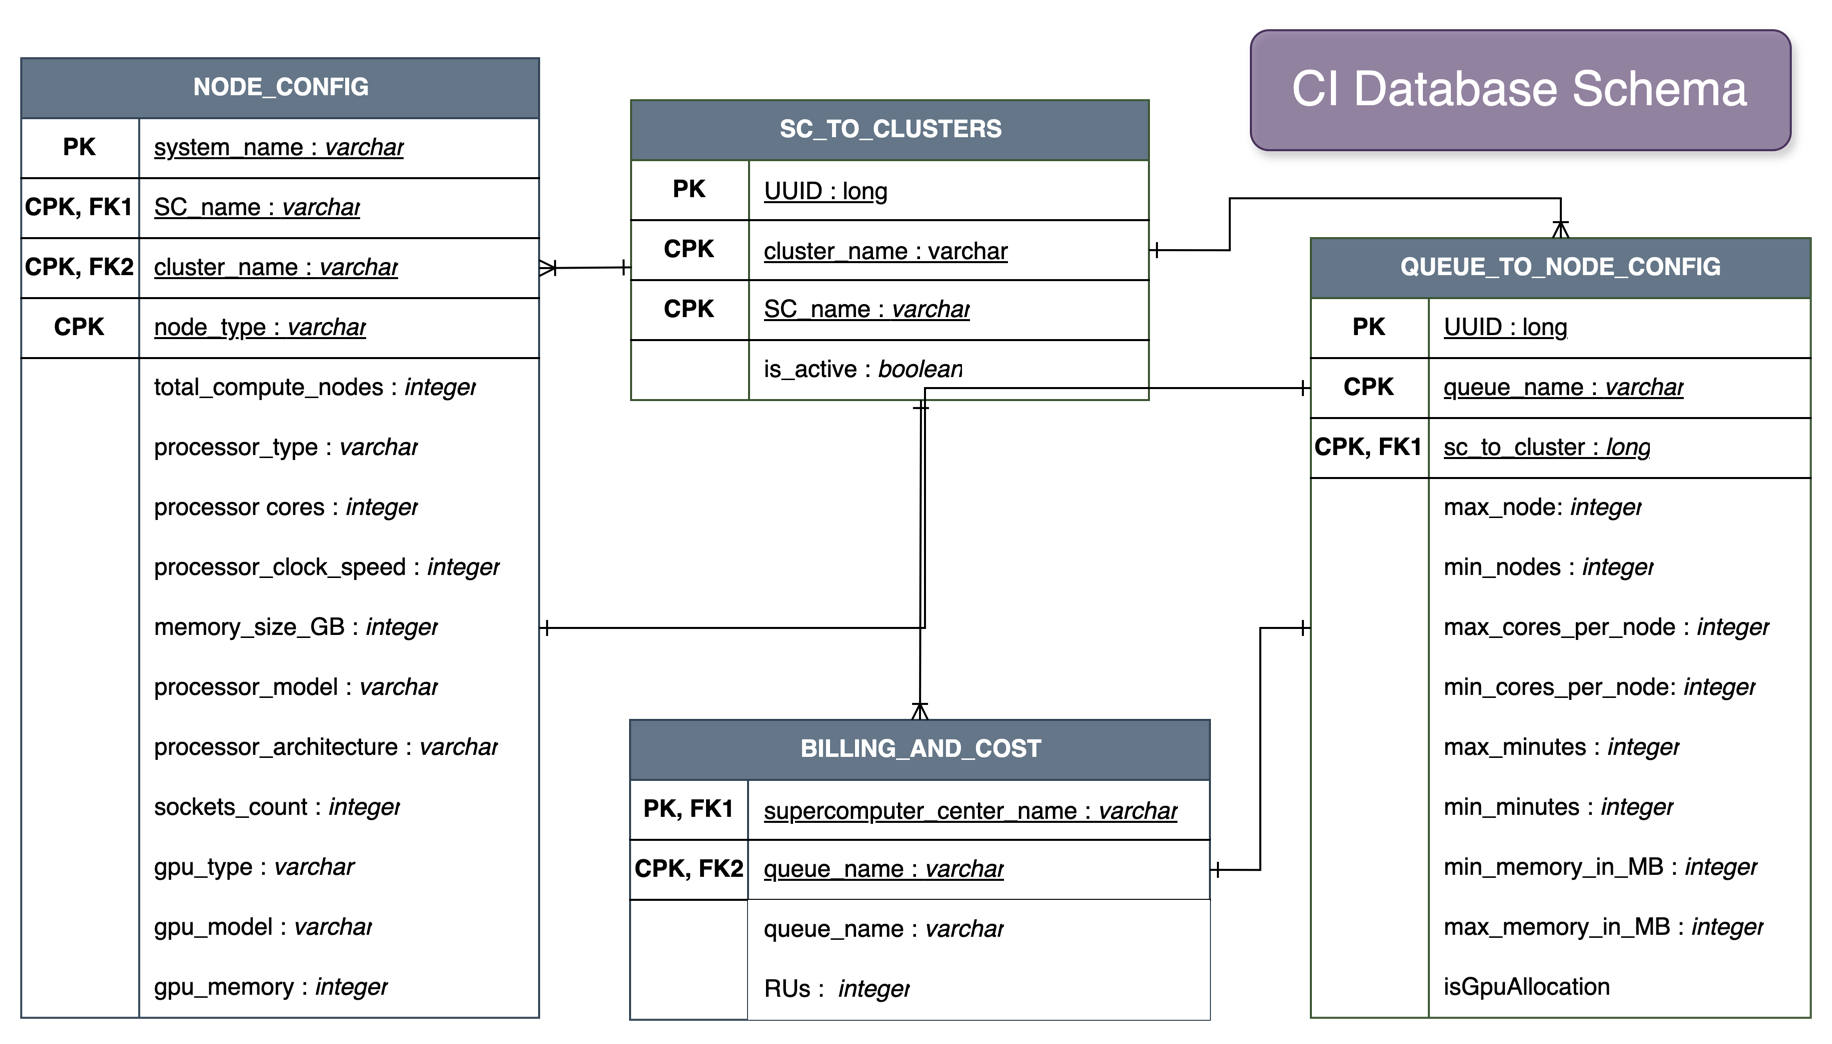
\includegraphics[width=0.9\textwidth]{Images/CIDBSchema.png}
    \caption{CI Database Schema. This schema represents the core components of the Cyberinfrastructure (CI) Database, including system configurations, queue properties, and billing details. The key tables include:
    \textit{SC\_TO\_CLUSTERS} maps supercomputing centers to their respective clusters.
    \textit{QUEUE\_TO\_NODE\_CONFIG} links job queues to their associated node batch limitations.
    \textit{NODE\_CONFIG} stores node-specific hardware configurations.
    \textit{BILLING\_AND\_COST} contains information about queue-based billing, including resource unit (RU) costs.
    This database enables efficient resource allocation, cost estimation, and feasibility validation for HPC job submissions.}
    \label{fig:ci_database_schema}
\end{figure}



\begin{table}[]
\centering
\caption{The table shows two cluster allocation policies at two supercomputing centers TACC lonestar6 and OSC Owens. *GPUs come with an additional cost of CPU cores per hour rate. }
\label{table:CIExamples}
\begin{tabular}{|crrr|}
\hline
\multicolumn{1}{|c|}{\textbf{\begin{tabular}[c]{@{}c@{}}Queue\\ Name\end{tabular}}} & \multicolumn{1}{c|}{\textbf{\begin{tabular}[c]{@{}c@{}}Min/Max \\ Nodes\\ per Job\end{tabular}}} & \multicolumn{1}{c|}{\textbf{\begin{tabular}[c]{@{}c@{}}Max Job \\ Duration \\ (Hrs)\end{tabular}}} & \multicolumn{1}{c|}{\textbf{\begin{tabular}[c]{@{}c@{}}Charge Rate \\ (per core per hour)\end{tabular}}} \\ \hline
\multicolumn{4}{|c|}{\textbf{TACC}} \\ \hline
\multicolumn{1}{|c|}{\textbf{development}} & \multicolumn{1}{r|}{4} & \multicolumn{1}{r|}{6} & 1 SU \\ \hline
\multicolumn{1}{|c|}{\textbf{gpu-a100}} & \multicolumn{1}{r|}{16} & \multicolumn{1}{r|}{16} & 4 SU \\ \hline
\multicolumn{1}{|c|}{\textbf{gpu-a100-dev}} & \multicolumn{1}{r|}{4} & \multicolumn{1}{r|}{2} & 4 SU \\ \hline
\multicolumn{1}{|c|}{\textbf{large}} & \multicolumn{1}{r|}{65/256} & \multicolumn{1}{r|}{256} & 1 SU \\ \hline
\multicolumn{1}{|c|}{\textbf{normal}} & \multicolumn{1}{r|}{1/64} & \multicolumn{1}{r|}{96} & 1 SU \\ \hline
\multicolumn{1}{|c|}{\textbf{vm-small}} & \multicolumn{1}{r|}{1} & \multicolumn{1}{r|}{4} & 0.143 SU \\ \hline
\multicolumn{4}{|c|}{\textbf{OSC}} \\ \hline
\multicolumn{1}{|c|}{serial} & \multicolumn{1}{r|}{1} & \multicolumn{1}{r|}{168} & \$0.003 \\ \hline
\multicolumn{1}{|c|}{parallel} & \multicolumn{1}{r|}{2/81} & \multicolumn{1}{r|}{96} & \$0.003 \\ \hline
\multicolumn{1}{|c|}{gpuserial} & \multicolumn{1}{r|}{1} & \multicolumn{1}{r|}{168} & \$0.009* \\ \hline
\multicolumn{1}{|c|}{gpuparallel} & \multicolumn{1}{r|}{2/8} & \multicolumn{1}{r|}{96} & \$0.009* \\ \hline
\multicolumn{1}{|c|}{\textbf{hugemem}} & \multicolumn{1}{r|}{1} & \multicolumn{1}{r|}{168} & \$0.004 \\ \hline
\multicolumn{1}{|c|}{debug} & \multicolumn{1}{r|}{1/2} & \multicolumn{1}{r|}{1} & \$0.003 \\ \hline
\end{tabular}
\end{table}

Figure~\ref{fig:ci_database_schema} illustrates the CI Database schema, which consists of system configurations, queue properties, and billing details. The CI Database Interface enhances this by applying rules on memory per CPU and cost per node-hour, enabling:

\begin{itemize}
    \item Resource Estimation
    \begin{itemize}
        \item Supports downstream applications for workload profiling against available system queues and node configurations. 
        \item Provides CPU, GPU, and memory specifications based on node configurations and queues to feed the resource estimators (inferencing)  
    \end{itemize}
    \item Allocation Feasibility Validation
    \begin{itemize}
        \item Ensures job requests align with hardware constraints before submission.
        \item Helps create execute options againt avaible queues and their feasibilities to enable smart schduling.
    \end{itemize}
    \item Cost Computation Against Batch Policies
    \begin{itemize}
        \item Applies cost models based on supercomputing center rules.
        \item Optimizes resource scheduling by balancing cost vs. execution efficiency.
    \end{itemize}
\end{itemize}


Table \ref{table:CIExamples} provides a snapshot of the CI configurations database, including selected columns from QUEUE\_TO\_NODE\_CONFIG and BILLING\_AND\_COST.


The CI Database is a critical component in HPC job optimization, providing a structured framework for resource-aware scheduling, cost estimation, and feasibility analysis. By evaluating resource requirements before job submission, it helps prevent non-feasible allocation requests, reducing the likelihood of jobs being rejected by SLURM checks or terminated due to errors such as out-of-memory issues. Additionally, the database facilitates the automatic generation of execution plans, including batch scripts, ensuring compliance with system policies while dynamically tuning resource requests based on estimator outputs.


